
\textcolor{blue} {\textit{Khadimoullah Vencatasamy}}

We want to simulate on a map and we want to generate the map easily. So the easiest way we found was to take a screen on Google earth where we know the scale.
Our objective is to transform this map into a binary image. To do so we choose to make a color filter to isolate the ground from the sea. We thought to use a contour filter but due to the many bumps present on the satellite view sea it was successful.

So we have a script which take a satellite view as input, when you run this script you have to windows: one with some trackbar which you can slide to filter the color you want and apply a closing filter  to erase the last parasite pixels. The second window show the output image. Press 's' to save the output image.

\begin{figure}[H]
\centering
  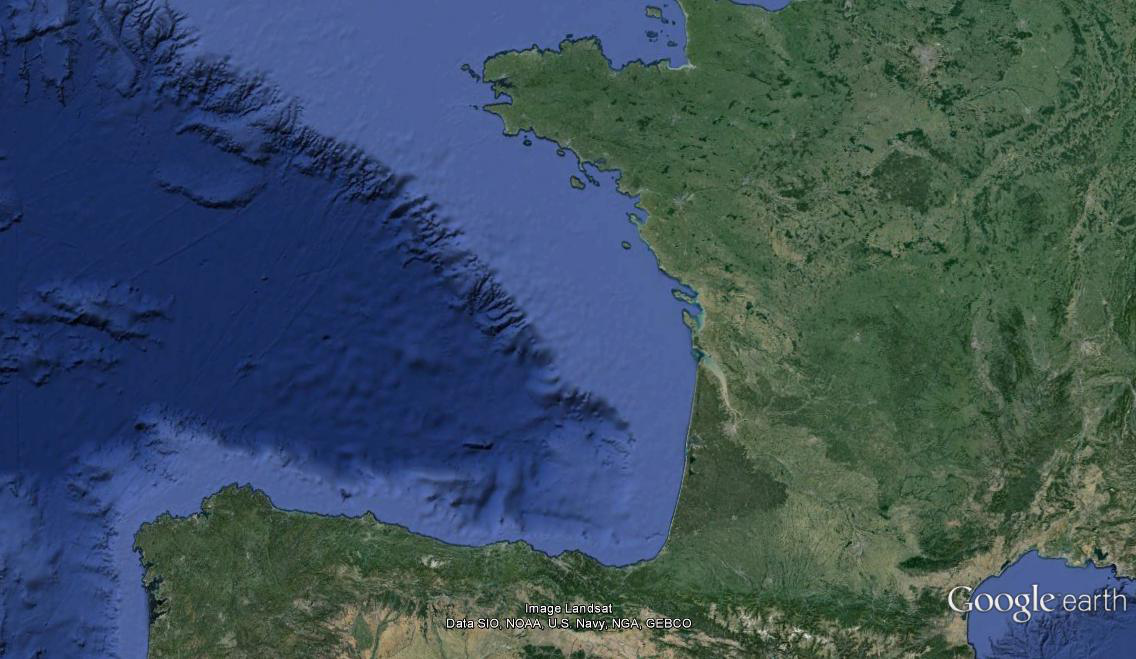
\includegraphics[width=0.6\linewidth]{GascogneSat.png}
  \caption{Input Image}
\end{figure}

\begin{figure}[H]
\centering
  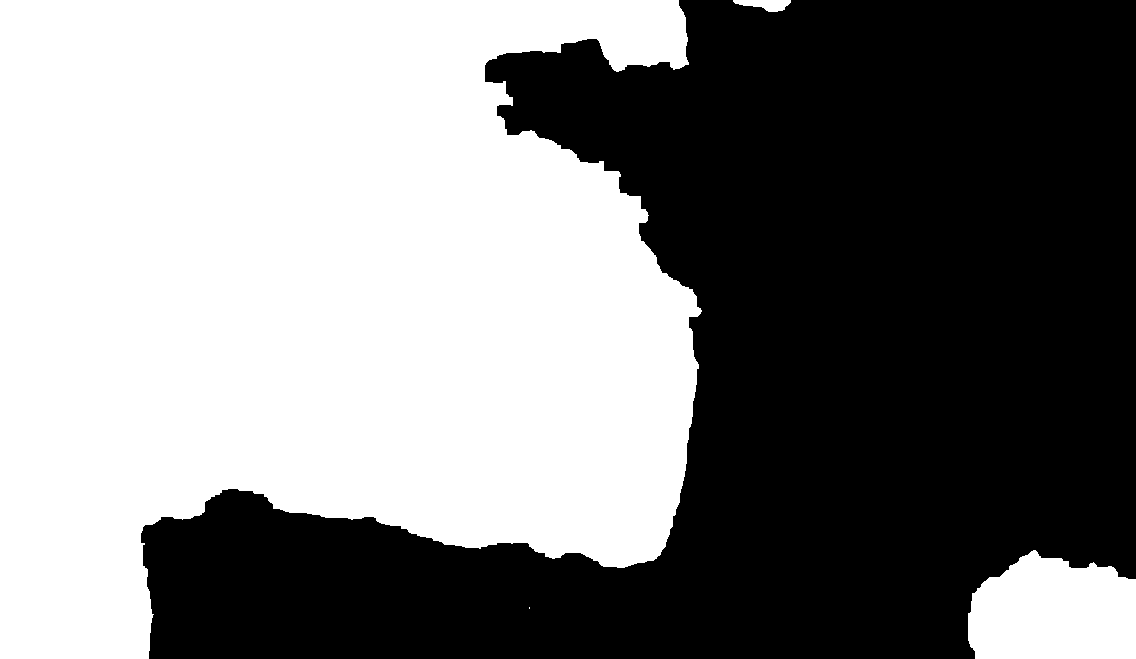
\includegraphics[width=0.6\linewidth]{BWFrance.png}
  \caption{Output Image}
\end{figure}


\begin{figure}[H]
\centering
  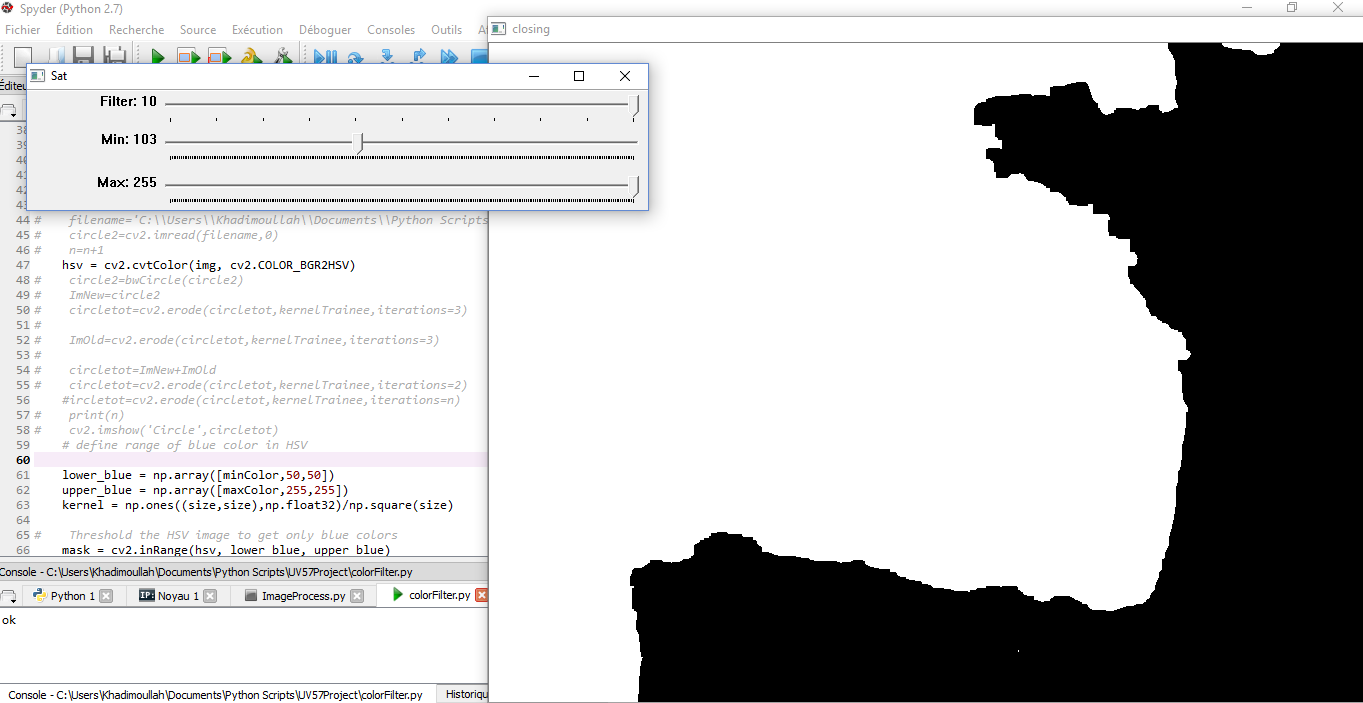
\includegraphics[width=0.6\linewidth]{BWFranceInterface.png}
  \caption{Interface to binarize the satellite image}
\end{figure}

This is this image which is use to generate the paving in ImageToBoxes script.

\subsection{Origin Determination}

In our problem we set the origin of the map to the point 45$^\circ$N 4$^\circ$W so we need to find the (i0,j0) which are the coordinates of the origin.

To achieve this we need the latitude and the longitude of the top left corner of our binary map.
We will note X Y for the coordinate in pixel and LAT LONG for the coordinate in WPs.

First let's determine the $\delta{X}$ and $\delta{Y}$:

%\begin{equation}
%\begin{case}
%\delta{X}=\frac{LONG2-LONG1}{X2-X1} & \text{ where LONG2 is the leftmost point and LONG1 is the rightmost point X1 and X2 is their X coordinate in pixel}\\
%\delta{Y}=\frac{LAT2-LAT1}{Y2-Y1} & \text{ where LAT2 is the	topmost point and LAT1 is the bottommost point Y1 and Y2 is their Y coordinate in pixel}\\
%\end{cases}\\
%\text{Lat0 and Long0 is the coordinate of the 0 0 pixel}\\
%\begin{case}
%LAT0=LAT1 -Y1 * \delta{Y} \\
%LONG0=LONG1 -X1 * \delta{X}\\
%\end{case}\\
%\text{We can now convert LAT/LONG to their pixel coordinate}\\
%\begin{case}
%X= \frac{LONG-LONG0}{\delta{X}}\\
%Y= \frac{LAT-LAT0}{\delta{Y}}\\ 
%\end{case}
%\end{equation}

In our case we have chosen (45$^\circ$N,4$^\circ$W) as origin which corresponds to the point (410 400) in pixel coordinate.

